\documentclass[11pt]{article}
\usepackage[margin=1in]{geometry}
\usepackage{amsmath,amssymb,booktabs,graphicx,microtype}
\usepackage{setspace,lineno,natbib,hyperref}
\hypersetup{hidelinks}
\usepackage[T1]{fontenc}
\usepackage{lmodern}
\usepackage[utf8]{inputenc}
\doublespacing
\linenumbers

\title{Urban boundaries and gender gaps in stochastic accessibility: Evidence from Bogotá}
\author{Andy Rafael Domínguez-Monterroza\\
Department of Mathematics, Pontificia Universidad Javeriana, Bogotá, Colombia\\
Corresponding author: \texttt{andy\_dominguez01@javeriana.edu.co}}
\date{}

\begin{document}
\maketitle

\begin{abstract}
Urban accessibility studies often use administrative boundaries to define both the mobility network and the population whose access is measured. We ask how this choice changes sex-disaggregated accessibility gaps in Bogotá and its surrounding municipalities. Survey-weighted origin--destination flows define regularized transition kernels, and first-passage times to employment, education, and health destinations summarize stochastic access. A paired household bootstrap shows larger female--male gaps in the complete regional system than in Bogotá D.C. for all three purposes. We then account separately for changing the network while retaining city residents and targets, changing purpose targets, and including regional residents. The first two contributions are small and their simultaneous intervals include zero; including residents outside the district accounts for most of the observed contrast. A four-scope analysis describes variation across intermediate boundaries without assuming a monotonic response. The results show how a district-only analysis can omit a substantial regional population gap, while the measured effect for district residents alone is less clearly distinguishable. These are descriptive comparisons of fitted aggregate mobility systems, not causal effects of administrative borders or estimates of individual travel time.
\end{abstract}

\noindent\textbf{Keywords:} urban accessibility; first-passage time; metropolitan boundaries; gender inequality; human mobility; Bogotá

\section{Introduction}
Accessibility links transport systems to the opportunities that people can reach and is therefore central to transport equity \citep{hansen1959,pereira2017}. Standard place-based indicators commonly combine a fixed travel cost with a cumulative or gravity-based opportunity function. These measures are useful for planning, but they usually treat connectivity as deterministic and take the study boundary as given. Sensitivity to spatial units is well established in the modifiable areal unit problem \citep{openshaw1983,fotheringham1991}; here the boundary also changes the network and population included in the estimand. In metropolitan systems, observed mobility repeatedly crosses administrative borders. An estimate restricted to the central municipality can therefore answer a materially different question from an estimate based on the functional urban region.

Gender is a particularly relevant dimension of this boundary problem. Individual space--time accessibility research has shown gender differences in access to opportunities \citep{kwan1999}, and mobility disparities have been mapped over administrative districts in Santiago \citep{gauvin2020}. Large-scale mobility studies have also documented differences in travel diversity, trip purpose, mode use, and exposure to urban infrastructure \citep{macedo2020,macedo2022,battiston2023}. For Colombia, previous analyses of Bogotá and Medellín show that these differences interact with socioeconomic status and the spatial distribution of destinations \citep{macedo2022}. Conventional potential-accessibility analysis has documented income- and mode-related inequalities in the Bogotá city-region \citep{guzman2017}. The distinct contribution here is to track how a subgroup accessibility gap changes when both the fitted mobility system and the included residential population expand beyond the district.

Random walks provide a natural language for studying access in complex networks. First-passage time (FPT) measures the expected number of transitions required to reach a target set \citep{noh2004} and has been used to characterize urban intelligibility and transport-constrained segregation \citep{blanchard2008,neira2024}. Related work uses random-walk coverage times to compare urban segregation across systems \citep{sousa2022}, while recent mobility studies quantify administrative and physical barriers \citep{pinter2025} and mode-specific layers of social mixing \citep{yang2026}. These studies establish the value of stochastic and behavior-sensitive representations, but they do not distinguish changing a mobility network from changing the population included in a territorial comparison. Unlike a shortest path, FPT depends on the full transition structure and therefore reflects the range and concentration of observed movements. Direct subgroup estimation remains vulnerable to sparse origin rows and unstable transition probabilities.

This paper defines stochastic accessibility to purpose-specific opportunity sets using weighted mobility-survey flows and regularizes group-specific transition rows according to their effective sample size. A paired design compares district and regional first-passage gaps under shared household bootstrap draws. A within-scope decomposition separates sex differences in residential distributions from differences in transition kernels; a separate ordered accounting distinguishes expansion of the fitted network, redefinition of destination sets, and inclusion of residents beyond the district. Four nested systems provide an exploratory view of the territorial response. The empirical question is which part of measured regional inequality a district-only analysis leaves outside its analytical population and mobility system.

\section{Data}
\subsection{Bogotá--Region Mobility Survey}
We use the processed microdata and 2023 zoning files from the official Bogotá--Region Household Mobility Survey \citep{eodh2023}. The public release contains linked household, person, trip, and trip-stage modules with survey expansion weights. The regional analytical sample retained 97,796 trips with valid household, origin, destination, and positive trip weight, and 64,373 persons whose residential unit belonged to the accepted network. The Bogotá D.C.-internal system retained 76,168 trips and 48,373 persons.

Spatial units are Urban Transport Analysis Units (UTAMs). The regional transition network contains 141 nodes. Bogotá D.C. contains 116 zoned UTAMs; the largest directed strongly connected component contains 114 nodes, 100\% of the internal trip weight, and 99.78\% of the eligible residential weight. The analysis uses the survey's reported binary sex categories (women and men). We use \emph{gender gap} for the observed association between these categories and mobility patterns, without claiming to measure gender identity or its causes. Results should not be generalized to identities not represented by these categories.

Figure~\ref{fig:study-area} shows the complete survey geography and the nested territorial scopes used in the multiscale analysis. External municipalities are classified according to the cumulative share of bidirectional survey-weighted flow that they exchange with Bogotá, using the full population before any subgroup comparison.

\begin{figure}[ht]
\centering
\IfFileExists{figures/figure_study_area_multiscale_scopes.png}{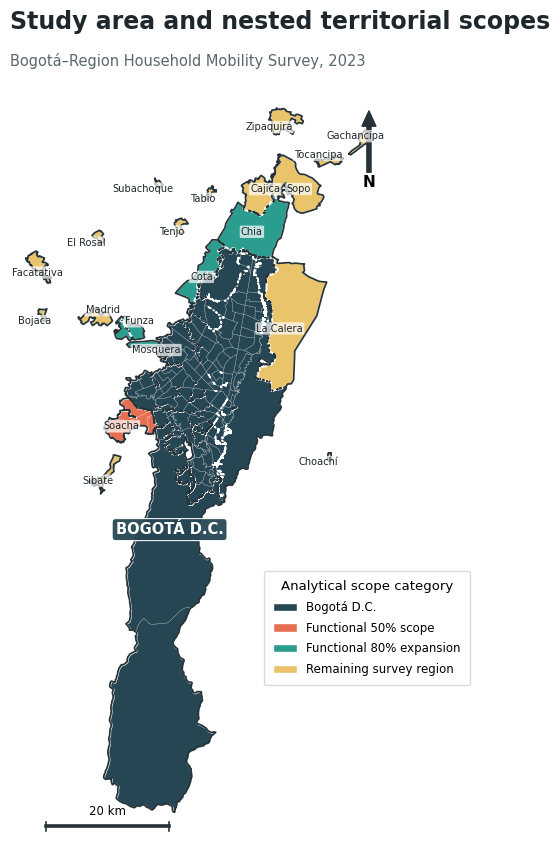
\includegraphics[width=0.94\textwidth,height=0.75\textheight,keepaspectratio]{figures/figure_study_area_multiscale_scopes.png}}{\fbox{\parbox[c][7cm][c]{0.88\textwidth}{\centering Generate figure\_study\_area\_multiscale\_scopes.png with notebook 17 and copy it to paper/figures/.}}}
\caption{Study area and nested territorial scopes in the Bogotá--Region Household Mobility Survey. Bogotá D.C. forms the administrative core; Soacha reaches the functional 50\% threshold; Mosquera, Chía, Funza, and Cota extend coverage beyond 80\% of observed Bogotá--external interface flow; the remaining municipalities complete the regional system. Thin internal lines show UTAM boundaries.}
\label{fig:study-area}
\end{figure}

\subsection{Purpose-specific opportunity sets}
Trip purposes were harmonized into employment, education, and health. For each purpose and territorial scope, destination UTAMs were ranked by weighted arrivals after requiring at least five sampled trips and an effective sample size of at least three. The primary target set is the smallest ranked set reaching 50\% of supported weighted arrivals (the \emph{core-50} definition). The district target sets contain 24 employment, 24 education, and 17 health UTAMs. Because targets are reconstructed inside each scope, the scope contrast captures the complete change in the measured mobility system, including its opportunity geography.

\section{Methods}
\subsection{Weighted mobility kernels}
Let $W_{ij}$ be the survey-weighted number of observed trips from UTAM $i$ to UTAM $j$. The population transition kernel is
\begin{equation}
 P^{(0)}_{ij}=\frac{W_{ij}}{\sum_k W_{ik}}.
\end{equation}
For group $g$, let $\widehat P^{(g)}$ be the corresponding empirical kernel and let
\begin{equation}
 \operatorname{ESS}^{(g)}_i=\frac{(\sum_{r\in i,g}w_r)^2}{\sum_{r\in i,g}w_r^2}
\end{equation}
be the effective sample size of trips leaving origin $i$. Sparse rows are regularized toward the population kernel:
\begin{equation}
 P^{(g)}_{ij}=\omega^{(g)}_i\widehat P^{(g)}_{ij}+
 (1-\omega^{(g)}_i)P^{(0)}_{ij},\qquad
 \omega^{(g)}_i=\frac{\operatorname{ESS}^{(g)}_i}{\operatorname{ESS}^{(g)}_i+\tau},
\end{equation}
with primary value $\tau=20$. At an origin with $\operatorname{ESS}^{(g)}_i=20$, the empirical group row and population row receive equal weight. We assess sensitivity over $\tau\in\{0,10,20,50\}$. The Markov chain describes aggregate population flows; its transitions are neither observed steps in an individual itinerary nor units of travel time.

\subsection{First-passage accessibility}
For target set $A$, let $T_A=\inf\{t\geq0:X_t\in A\}$. The vector of mean first-passage times $h^{(g,A)}$ is zero on $A$ and satisfies
\begin{equation}
 h_{-A}^{(g,A)}=\mathbf 1+Q^{(g,A)}h_{-A}^{(g,A)},
 \qquad
 h_{-A}^{(g,A)}=(I-Q^{(g,A)})^{-1}\mathbf 1,
\end{equation}
where $Q^{(g,A)}$ is the transient submatrix of $P^{(g)}$. Let $\mu^{(g)}$ be the survey-weighted residential distribution for group $g$, conditioned on starting outside $A$. Group accessibility is summarized as
\begin{equation}
 M^{(g,A)}=\mu^{(g)\top}h^{(g,A)}.
\end{equation}
Larger values indicate more expected mobility transitions before reaching the opportunity set and hence lower stochastic accessibility.

\subsection{Residence--kernel decomposition}
For women ($w$) and men ($m$), the total gap is $G=M^{(w,A)}-M^{(m,A)}$. To distinguish a change in the gap from a general change in the FPT scale, we also report the descriptive normalized gap
\begin{equation}
 G_{\mathrm{rel}}=
 \frac{M^{(w,A)}-M^{(m,A)}}
 {\{M^{(w,A)}+M^{(m,A)}\}/2}.
\end{equation}
Inference is based on the primary absolute gap $G$; $G_{\mathrm{rel}}$ is used as a scale-comparability diagnostic. We use a symmetric two-factor decomposition:
\begin{align}
 R &= \tfrac12(\mu^w-\mu^m)^\top(h^w+h^m),\\
 K &= \tfrac12(\mu^w+\mu^m)^\top(h^w-h^m),
\end{align}
so that $G=R+K$. Here $R$ is associated with the residential starting distribution and $K$ with differences in transition dynamics. The decomposition is algebraic and descriptive; it is not a causal mediation analysis.

To distinguish changes in the estimated territorial gap from changes in the population represented, we also compute four ordered states. $G_D$ uses district kernels, district purpose targets, and residents of the 114-node district component. $G_{RC}$ uses regional kernels while retaining those residents and district purpose targets. $G_{RT}$ retains the same residents and regional kernels but uses regional targets. $G_R$ uses regional kernels, targets, and all eligible regional residents. For every state and sex, the residential distribution is normalized after excluding the relevant destination set. The exact identity
\begin{equation}
G_R-G_D=(G_{RC}-G_D)+(G_{RT}-G_{RC})+(G_R-G_{RT})
\label{eq:territorial-accounting}
\end{equation}
attributes the endpoint difference, in this order, to a change in the fitted mobility network, a change in the target set, and an expanded residential population. The first term includes the refitting of transition probabilities on the regional network; the three terms are descriptive and depend on the specified order. In 500 additional shared household-bootstrap replicates, these four states receive identical Poisson(1) household multipliers. The connected components, population reference kernels, and target sets remain fixed during inference. Max-$t$ intervals are simultaneous across the three purposes within each term, separately. This accounting is distinct from the within-scope $R+K$ decomposition.

\subsection{Multiscale territorial-scope response and inference}
We construct four nested mobility systems. The first retains trips, residences, and targets internal to Bogotá D.C. External municipalities are then ranked by their total bidirectional survey-weighted flow with Bogotá, using the complete population and without reference to sex or outcomes. The functional 50\% and functional 80\% systems add the smallest ranked sets reaching at least 50\% and 80\% of this interface flow; the fourth system is the complete Bogotá--Region network. The realized interface shares are $q_s\in\{0,0.564,0.824,1\}$. Within every scope, the largest directed strongly connected component, population kernel, residential distributions, and core-50 purpose targets are reconstructed.

For each purpose, the endpoint contrast is
\begin{equation}
 \Delta_{\mathrm{scope}}=G_{\mathrm{region}}-G_{\mathrm{district}},
\end{equation}
and the multiscale response is summarized by the ordinary least-squares slope $\beta$ in
\begin{equation}
 G_s=\alpha+\beta q_s+\varepsilon_s,
\end{equation}
evaluated over the four constructed realized shares. A positive $\beta$ indicates that the measured gender gap tends to increase as observed metropolitan interface flow is incorporated. This slope summarizes the constructed scopes and is not a causal or continuous boundary effect.

Sampling uncertainty is estimated with a joint Poisson(1) household-cluster bootstrap. Each of 500 replicates assigns one multiplier to every household and applies it simultaneously to person and trip records in all four territorial scopes. Pointwise percentile intervals and max-$t$ simultaneous intervals across the three destination purposes are reported separately for the total gap, residential component, and kernel component. Scope-specific target sets and population shrinkage kernels are reconstructed at the point-estimate stage and held fixed during bootstrap inference.

Two additional diagnostics probe the interpretation of the primary endpoint contrast. First, a time-threshold accessibility proxy uses pooled, survey-weighted mean reported duration for observed directed origin--destination edges, the shortest travel-time path to each supported core-50 destination UTAM, and pooled weighted destination arrivals as opportunity weights. For women and men separately, we average the share of weighted destinations reachable within 45 or 60 minutes over their residential distributions, conditional on starting outside the target set. We define female disadvantage as male minus female reachable share. Paired regional-minus-district benchmark contrasts receive percentile intervals from 500 shared Poisson household resamples with fixed pooled travel-time surfaces and destinations. This benchmark describes revealed OD connectivity and does not contain a group-specific transition kernel.

Second, we recompute the sex-specific empirical transition rows using only trips that depart from each household's residential UTAM, keeping the full population reference kernel, purpose targets, network components, and residential distributions fixed. These home-origin results are point-estimate sensitivities. Finally, to probe uncertainty from target selection, we perform 150 additional paired household resamples with and without rebuilding the core-50 destination sets within each replicate. Both variants retain the original network components and population reference kernel, and their percentile intervals are exploratory rather than substitutes for the primary simultaneous max-$t$ intervals.

\section{Results}
\subsection{Gender gaps within each territorial scope}
In Bogotá--Region, the female-minus-male mean FPT gap was 0.999 steps for employment (simultaneous 95\% confidence interval [0.632, 1.366]), 0.827 for education [0.451, 1.204], and 0.705 for health [0.252, 1.159]. The corresponding Bogotá D.C.-internal estimates were 0.479 [0.289, 0.669], 0.399 [0.173, 0.624], and 0.240 [-0.046, 0.527]. Thus, the sign is consistent across all point estimates, although the district health gap does not exclude zero after family-wise correction.

Table~\ref{tab:fpt-levels} reports the group-specific levels underlying these differences. After normalization by the two-group mean FPT, the employment gap increased from 12.4\% within Bogotá D.C. to 21.7\% in Bogotá--Region. The corresponding changes were from 10.0\% to 17.5\% for education and from 4.7\% to 10.7\% for health. The regional amplification therefore remains present on the relative scale and is not solely a consequence of higher overall FPT levels. These normalized quantities are descriptive diagnostics and are not assigned the confidence intervals of the absolute gaps.

\begin{table}[ht]
\centering
\caption{Group-specific mean FPT levels and female-minus-male gaps on absolute and normalized scales. Relative gaps divide the absolute gap by the two-group mean FPT.}
\label{tab:fpt-levels}
\begin{tabular}{llrrrr}
\toprule
Scope & Purpose & Men & Women & Absolute gap & Relative gap (\%) \\
\midrule
Bogotá D.C. & Employment & 3.616 & 4.095 & 0.479 & 12.4 \\
Bogotá--Region & Employment & 4.111 & 5.110 & 0.999 & 21.7 \\
Bogotá D.C. & Education & 3.789 & 4.187 & 0.399 & 10.0 \\
Bogotá--Region & Education & 4.306 & 5.133 & 0.827 & 17.5 \\
Bogotá D.C. & Health & 5.045 & 5.285 & 0.240 & 4.7 \\
Bogotá--Region & Health & 6.257 & 6.963 & 0.705 & 10.7 \\
\bottomrule
\end{tabular}
\end{table}

The residential contribution was close to zero in every scope-purpose combination and all of its simultaneous intervals included zero. In contrast, the mobility-kernel contribution closely reproduced the total gap. Figure~\ref{fig:scope} summarizes the scope-specific estimates.

\begin{figure}[ht]
\centering
\IfFileExists{figures/figure_1_scope_sex_gaps.png}{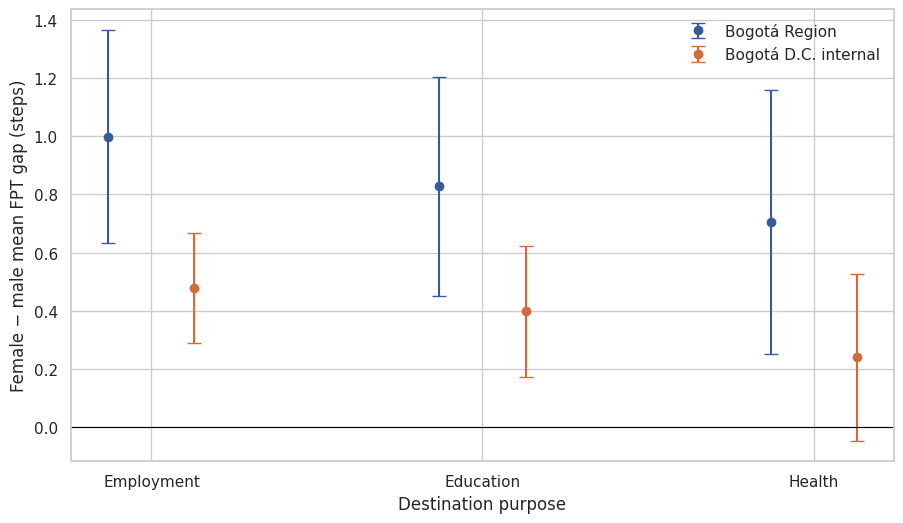
\includegraphics[width=0.9\textwidth]{figures/figure_1_scope_sex_gaps.png}}{\fbox{\parbox[c][5cm][c]{0.85\textwidth}{\centering Copy figure\_1\_scope\_sex\_gaps.png from Gate 14 to paper/figures/.}}}
\caption{Gender gaps in stochastic accessibility by territorial scope}
\label{fig:scope}
\end{figure}

\subsection{Paired metropolitan amplification}
The regional-minus-district gap was 0.520 steps for employment (simultaneous 95\% confidence interval [0.178, 0.861]), 0.429 for education [0.070, 0.787], and 0.465 for health [0.087, 0.843]. Restricting the system to Bogotá D.C. attenuated the point estimates by 52.0\%, 51.8\%, and 65.9\%, respectively. All three paired contrasts remained positive under simultaneous correction.

Kernel contrasts were likewise positive for employment (0.542 [0.217, 0.866]), education (0.451 [0.108, 0.794]), and health (0.495 [0.136, 0.853]). Residential contrasts were small and their intervals included zero. The within-scope residence--kernel decomposition associates the gap with fitted transition kernels (Figure~\ref{fig:contrast}); it does not separate extending the territorial network from including residents of additional municipalities. We address that distinction below.

This conclusion was stable in point-estimate sensitivity analyses over $\tau\in\{0,10,20,50\}$. The regional-minus-district total-gap contrast ranged from 0.472 to 0.557 steps for employment, from 0.380 to 0.468 for education, and from 0.423 to 0.497 for health. Kernel contrasts remained positive throughout, residential contrasts remained small, and all regional-minus-district relative-gap contrasts were positive. These calculations assess point-estimate sensitivity; the simultaneous intervals refer to the primary $\tau=20$ specification (Additional file 1, Table~S1).

The scope contrast also remained positive across all 12 effective combinations of target definition, residential conditioning, and purpose. Its range was 0.033--0.520 steps for employment, 0.034--0.429 for education, and 0.368--0.699 for health. Kernel and relative-gap contrasts were positive in every combination. The wide ranges, particularly for employment and education, show that target breadth and residential conditioning affect magnitude even though they do not reverse the observed metropolitan amplification (Additional file 1, Table~S10).

\begin{figure}[ht]
\centering
\IfFileExists{figures/figure_2_paired_scope_amplification.png}{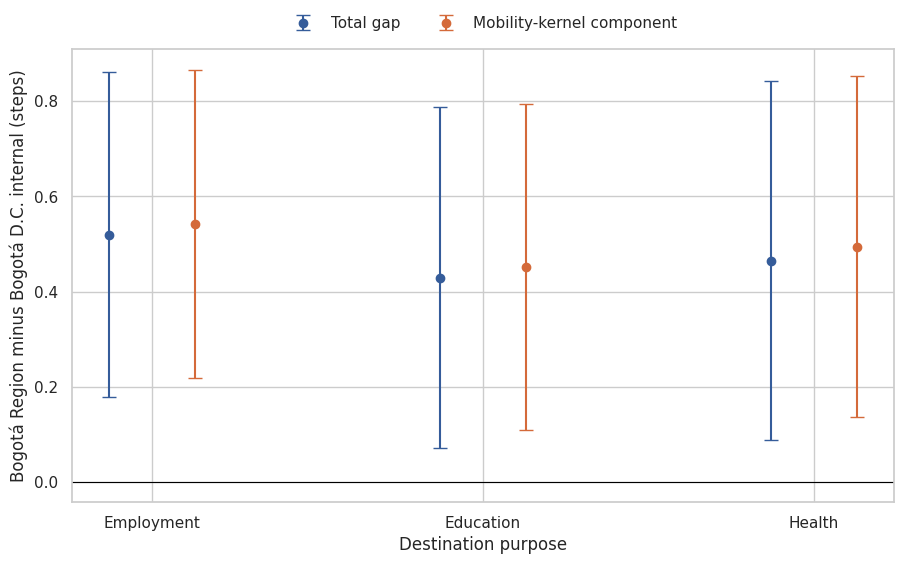
\includegraphics[width=0.9\textwidth]{figures/figure_2_paired_scope_amplification.png}}{\fbox{\parbox[c][5cm][c]{0.85\textwidth}{\centering Copy figure\_2\_paired\_scope\_amplification.png from Gate 14 to paper/figures/.}}}
\caption{Paired amplification of gender gaps at regional scale}
\label{fig:contrast}
\end{figure}

\subsection{Multiscale boundary response}
The four-scope analysis reveals a positive overall response to metropolitan expansion, but not strict stepwise monotonicity for every purpose. Employment gaps increased from 0.479 in Bogotá D.C. to 0.698 at functional 50\%, 0.722 at functional 80\%, and 0.999 in the complete region. Education gaps were 0.399, 0.335, 0.434, and 0.827, while health gaps were 0.240, 0.486, 0.434, and 0.705.

The estimated total-gap slope per unit of interface-flow coverage was 0.451 for employment (simultaneous 95\% confidence interval [0.161, 0.741]), 0.320 for education [0.024, 0.616], and 0.391 for health [0.052, 0.730]. The corresponding kernel-component slopes were 0.469 [0.175, 0.762], 0.338 [0.035, 0.641], and 0.417 [0.078, 0.755]. Residential-component slope intervals all included zero. Bootstrap probabilities of a fully nondecreasing sequence across the four scopes were 0.756 for employment, 0.110 for education, and 0.212 for health. Accordingly, the supported claim is a positive average boundary response across constructed scopes, not universal local monotonicity. Figures~\ref{fig:multiscale} and~\ref{fig:multiscale-decomposition} show the total and decomposed responses.

\begin{figure}[ht]
\centering
\IfFileExists{figures/figure_boundary_response_total_gap.png}{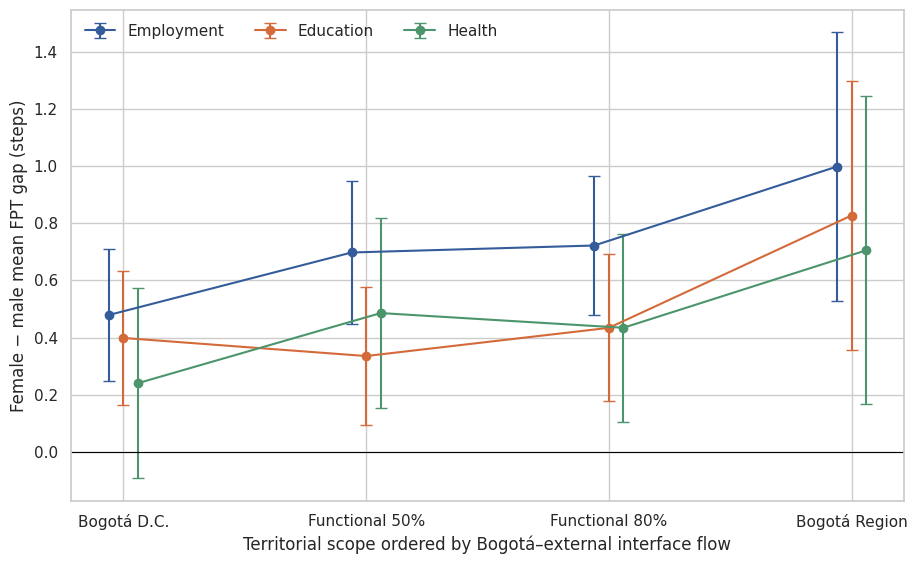
\includegraphics[width=0.9\textwidth]{figures/figure_boundary_response_total_gap.png}}{\fbox{\parbox[c][5cm][c]{0.85\textwidth}{\centering Copy figure\_boundary\_response\_total\_gap.png from Gate 16 to paper/figures/.}}}
\caption{Multiscale response of the female--male stochastic-accessibility gap to progressively broader functional territorial scopes. Points show scope estimates; uncertainty and fitted slopes are obtained from the shared household-cluster bootstrap.}
\label{fig:multiscale}
\end{figure}

\begin{figure}[ht]
\centering
\IfFileExists{figures/figure_boundary_response_decomposition.png}{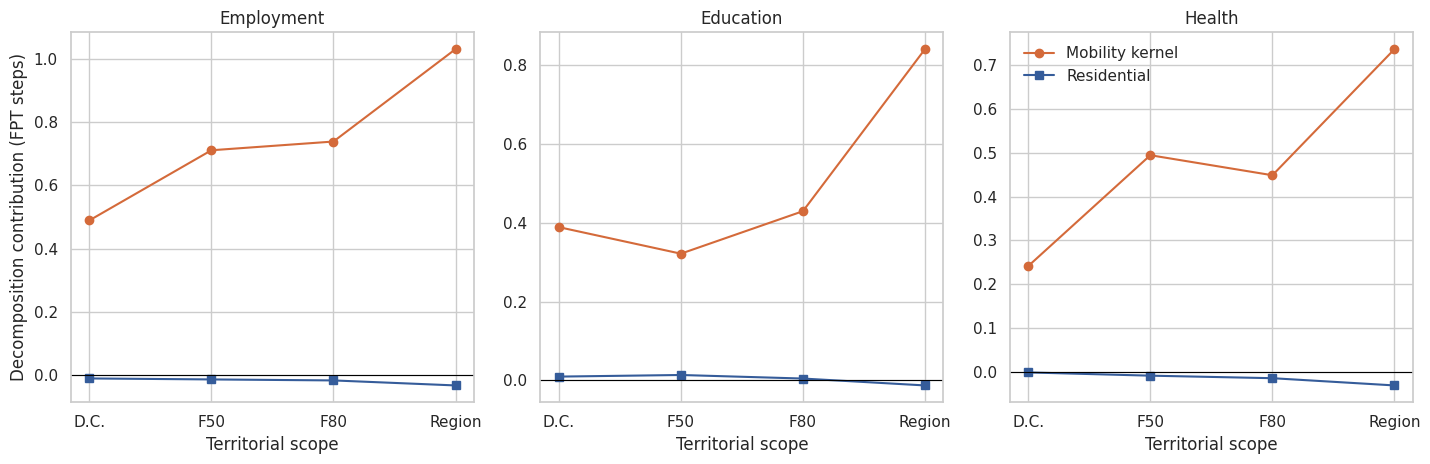
\includegraphics[width=0.96\textwidth]{figures/figure_boundary_response_decomposition.png}}{\fbox{\parbox[c][5cm][c]{0.9\textwidth}{\centering Copy figure\_boundary\_response\_decomposition.png from Gate 16 to paper/figures/.}}}
\caption{Multiscale decomposition of the territorial boundary response}
\label{fig:multiscale-decomposition}
\end{figure}

\subsection{Municipal contributions}
Among external municipalities, Facatativá had the largest positive kernel contribution for all three opportunity classes: 0.223 steps for employment, 0.308 for education, and 0.185 for health. Soacha contributed 0.204 for employment and 0.172 for health, while its education contribution was slightly negative. These are additive origin-level attributions under the fitted regional model, not effects of deleting municipalities. In particular, leave-one-municipality-out residential calculations retain the regional kernel and must not be interpreted as infrastructure interventions. Figure~\ref{fig:municipal-contributions} displays the purpose-specific external-municipality attributions.

A separate full-refit diagnostic excluded each of the 20 external municipalities in turn and reconstructed the regional network, both sex-specific kernels, residential distributions, and purpose-specific targets. The regional-minus-district gap remained positive after every omission: 0.277--0.565 steps for employment, 0.080--0.564 for education, and 0.270--0.552 for health. Excluding Facatativá yielded the smallest contrast for each purpose, with 0.277, 0.080, and 0.270 steps, respectively; it had 229 sampled outbound households. Excluding Soacha yielded 0.389, 0.560, and 0.347 steps, respectively, with 1,449 sampled outbound households. The regional-minus-district normalized-gap contrast also remained positive after every omission. These are point-estimate influence diagnostics: the confidence intervals for the primary analysis cannot be transferred to the refitted networks (Additional file 1, Table~S11).

\begin{figure}[ht]
\centering
\IfFileExists{figures/figure_3_external_municipality_kernel_contributions.png}{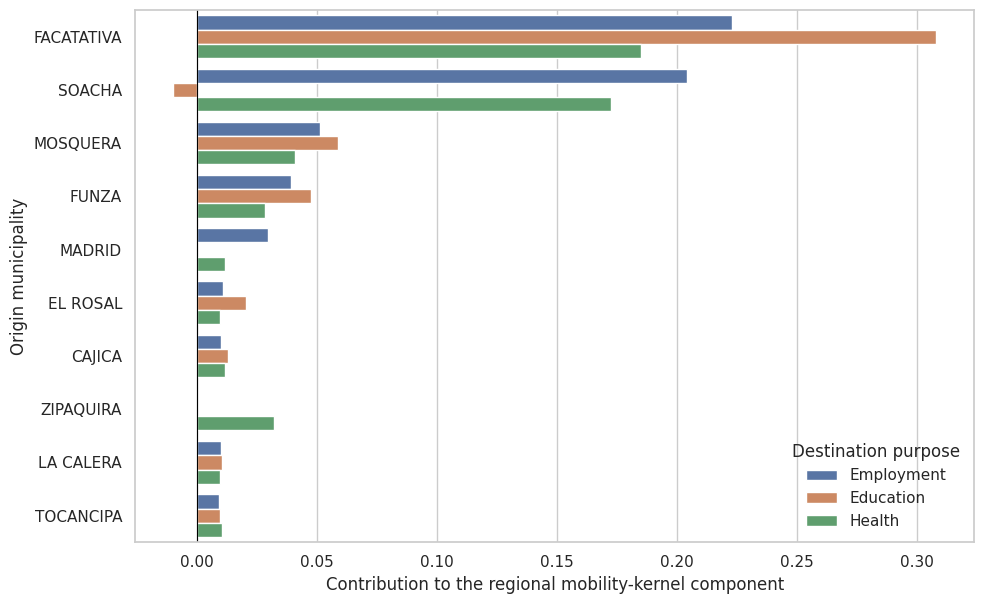
\includegraphics[width=0.94\textwidth]{figures/figure_3_external_municipality_kernel_contributions.png}}{\fbox{\parbox[c][5cm][c]{0.88\textwidth}{\centering Copy figure\_3\_external\_municipality\_kernel\_contributions.png from Gate 14 to paper/figures/.}}}
\caption{External-municipality contributions to the regional mobility-kernel component}
\label{fig:municipal-contributions}
\end{figure}

\subsection{Comparison with time-based accessibility and home-origin kernels}
The deterministic time-threshold proxy showed regional-minus-district female-disadvantage contrasts between -0.0008 and -0.0028 in weighted reachable-opportunity share across the three purposes and two thresholds. Five of six descriptive bootstrap percentile intervals included zero; the education contrast at 45 minutes was -0.0028 [-0.0054, -0.0001]. These shares cannot be compared numerically with FPT transitions. In this pooled-time benchmark, sex differences arise from residential starting distributions alone, whereas the FPT analysis also incorporates sex-specific transition patterns. The distinct boundary responses indicate that the two operational measures summarize different features of the observed system, without establishing that one is a more accurate measure of real opportunities (Additional file 1, Table~S12).

When empirical female and male kernel rows were restricted to home-origin trips, the regional-minus-district FPT contrasts remained positive at 0.558, 0.504, and 0.333 transitions for employment, education, and health, respectively, compared with 0.520, 0.429, and 0.465 in the primary model. Home-origin trips represented 62.3\% of pooled survey-weighted regional trips. This point-estimate diagnostic shows that non-home departures alone do not generate the sign of metropolitan amplification; it does not remove all trip chaining or identify its behavioral cause (Additional file 1, Table~S12).

In the reduced paired bootstrap, reselecting destination sets yielded exploratory percentile intervals of [0.184, 0.799] for employment, [0.050, 0.904] for education, and [0.048, 0.928] for health. All remained above zero, but the education and health intervals widened relative to fixed targets while the employment interval narrowed. These 150-replicate intervals are unadjusted across purposes and do not replace the primary 500-replicate simultaneous intervals (Additional file 1, Table~S13). Figure~\ref{fig:gate23-validation} displays these three distinct diagnostics without equating their units or interval definitions.

\begin{figure}[p]
\centering
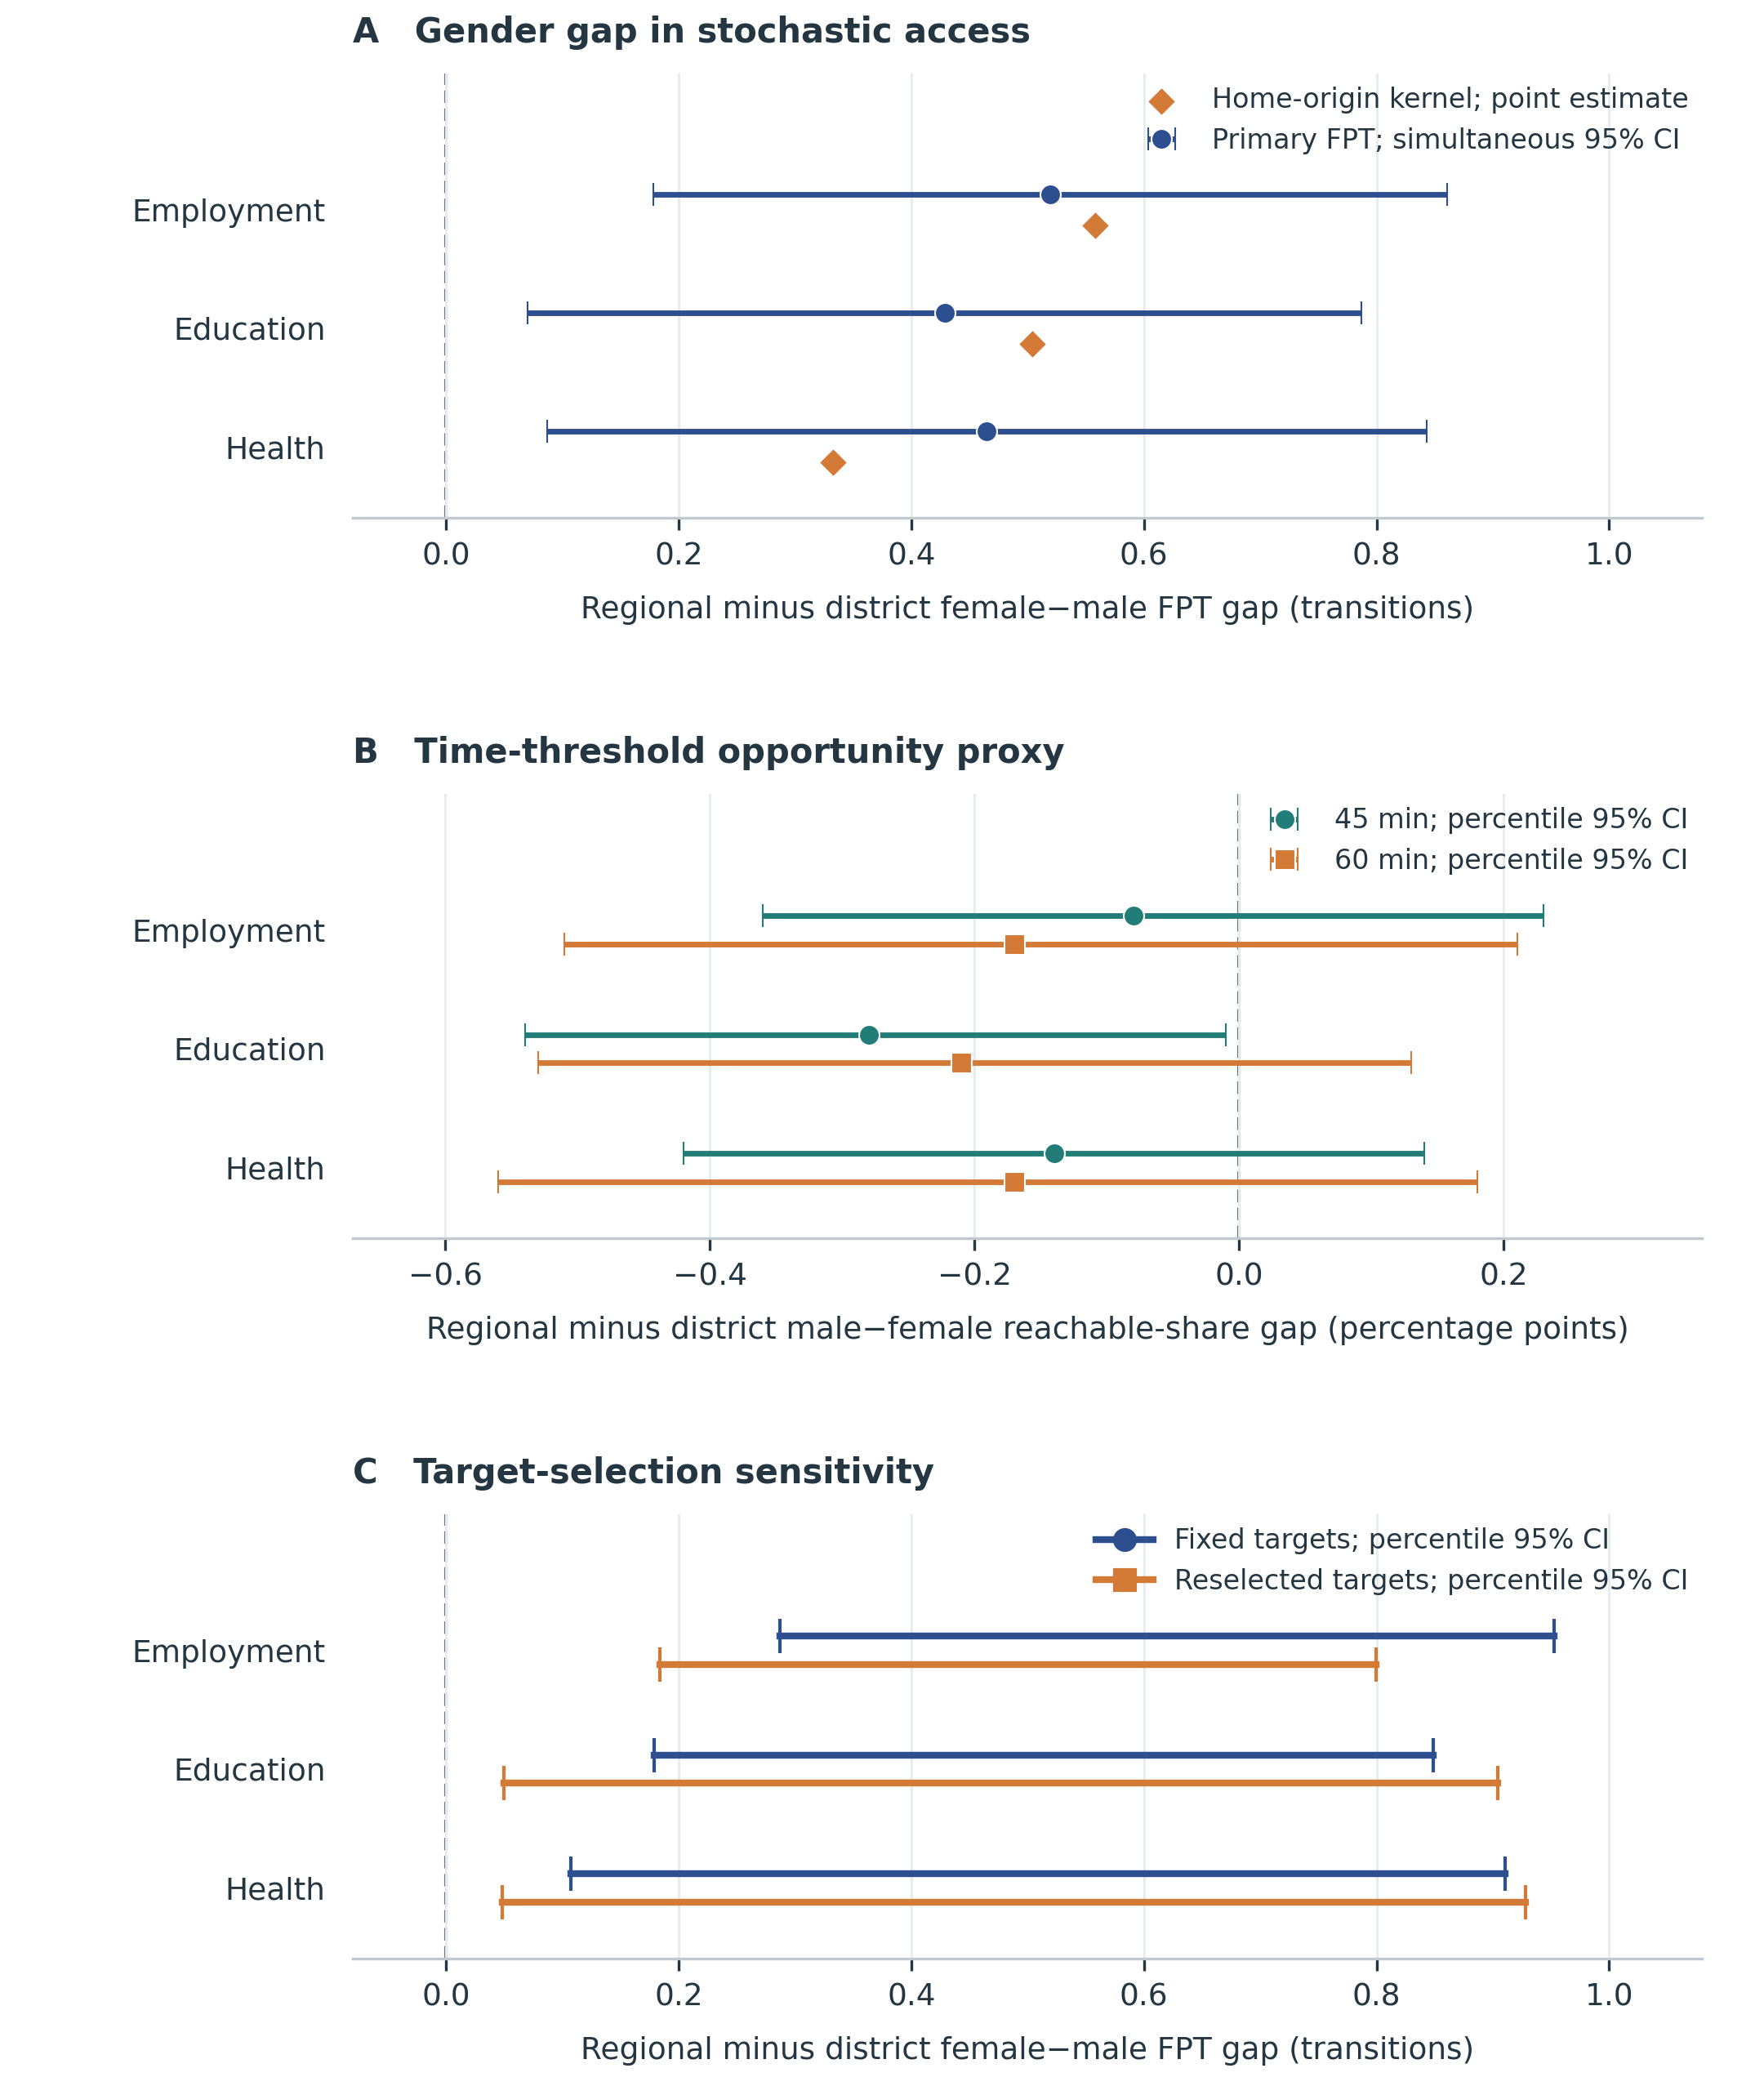
\includegraphics[width=0.95\textwidth]{figures/figure_7_validation_diagnostics.png}
\caption{Sensitivity diagnostics for the regional gender gap in stochastic access. (A) Primary regional-minus-district first-passage-time (FPT) contrast and its simultaneous 95\% confidence interval, alongside a home-origin-only point estimate. (B) Regional-minus-district contrast in the weighted share of destinations reachable within 45 or 60 minutes; conditional percentile intervals are descriptive and unadjusted. (C) Exploratory 150-replicate conditional percentile intervals for fixed and reselected opportunity sets. Each panel has its own units; panel C does not replace the primary inference in panel A.}
\label{fig:gate23-validation}
\end{figure}

\subsection{Separating territorial changes in network, destinations, and residents}
Equation~\ref{eq:territorial-accounting} separates the original endpoint contrast without changing its point estimates. The fitted network change, evaluated for residents of the district component against the district target set, contributed 0.015 transitions for employment (simultaneous 95\% confidence interval [-0.051, 0.082]), 0.052 for education [-0.031, 0.136], and -0.027 for health [-0.119, 0.065]. Replacing district targets with regional targets while retaining those same residents contributed 0.002 [-0.102, 0.106], -0.056 [-0.195, 0.083], and 0.001 [-0.109, 0.110], respectively. All six intervals include zero.

Adding the eligible residents outside the district to the regional model contributed 0.502 transitions for employment [0.156, 0.848], 0.433 for education [0.090, 0.775], and 0.491 for health [0.138, 0.845]. These positive contributions account for most of the observed regional-minus-district point contrast. The three ordered terms sum to 0.520, 0.429, and 0.465 transitions, respectively, with rounding. Figure~\ref{fig:boundary-mechanism} and Supplementary Table~S14 display the accounting. Its newly computed total intervals arise from a separate bootstrap run and do not replace the primary intervals in Supplementary Table~S7.

\begin{figure}[p]
\centering
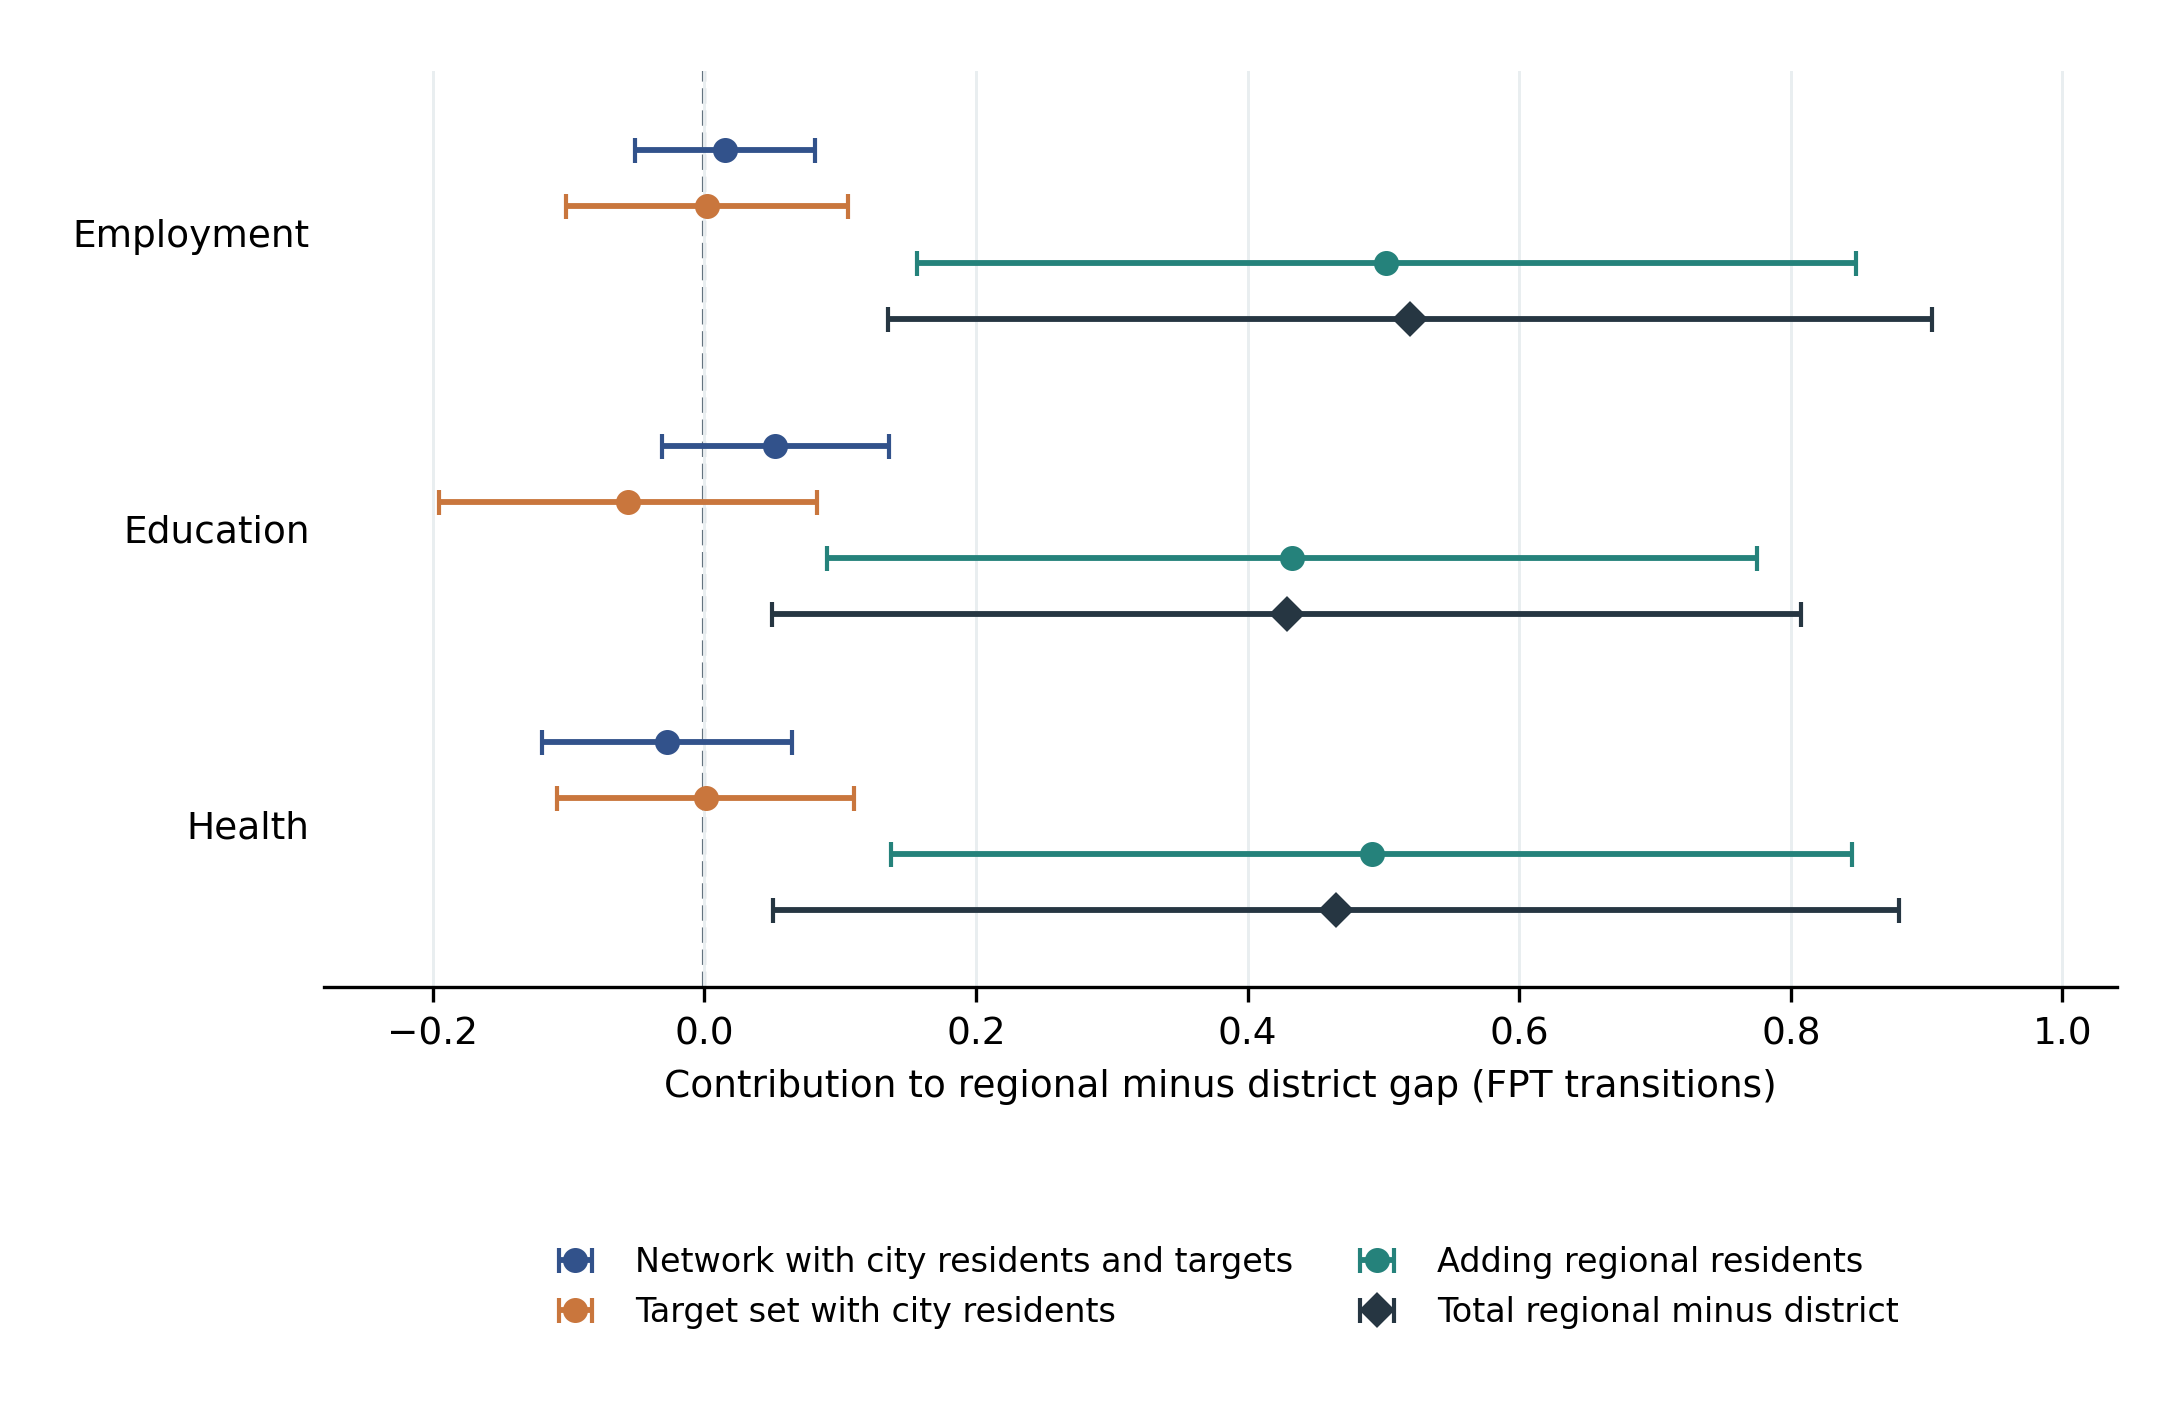
\includegraphics[width=0.96\textwidth]{figures/figure_boundary_mechanism.png}
\caption{Ordered contributions to regional-minus-district first-passage gaps. The district uses district residents, targets, and kernels. Moving to regional kernels while retaining district residents and targets is followed by changing to regional targets and then including the regional residential population. Points are descriptive contributions in expected transitions; bars are 95\% max-$t$ intervals simultaneous across the three purposes within each contrast separately. The three contributions sum to the endpoint contrast; they are conditional on the specified order and are not causal effects.}
\label{fig:boundary-mechanism}
\end{figure}

\section{Discussion}
The paired result is a difference between two territorial populations and fitted mobility systems: Bogotá D.C. has a smaller female--male FPT gap than the surrounding region for all three purposes. This extends evidence on accessibility inequities in Bogotá \citep{guzman2017} and spatial patterns of gendered mobility in other Latin American metropolitan regions \citep{gauvin2020,macedo2022}. The ordered accounting sharpens its meaning. With district residents held fixed, substituting regional kernels or regional destinations produces small, imprecisely estimated contrasts. Adding regional residents contributes most of the observed difference. Thus the district-only result primarily omits a disparity associated with the external residential population; it provides limited evidence for a sizeable change in the district residents' measured gap when their fitted network alone expands. Relative gap levels likewise increase between endpoints, while intermediate education and health scopes do not form a monotonic sequence. Fitted slopes describe these four constructed scopes and reuse the endpoint data; they are not independent confirmation of the paired finding.

The municipality omission diagnostic indicates that no single external municipality reverses the endpoint point contrast. Omitting Facatativá reduces the education contrast to 0.080 transitions from 0.429, so that purpose's magnitude is particularly sensitive to this municipality. The refit changes network flows, sampled residences, and destinations together; it does not identify a municipality's causal contribution. The sign also persists across the shrinkage range and the 12 target-and-residence specifications, although employment and education estimates approach zero when the target sets widen. The magnitude therefore depends materially on the chosen opportunity definition.

The two decompositions answer different questions. Within a fixed scope, the female--male gap lies mainly in the fitted transition-kernel component, and the residential-distribution component is small. Across scopes, the regional system also includes peripheral residents whose starting UTAMs and fitted transition patterns differ from those of district residents. Their addition is the principal term in the ordered accounting. A small within-scope residential component therefore does not imply that the composition of the analytical population is irrelevant to the territorial comparison. These descriptive patterns are compatible with documented gendered differences in trip purpose, mobility diversity, mode use, and constraints \citep{macedo2020,macedo2022,battiston2023}, without identifying their behavioral causes.

The time-threshold comparator yields near-zero or negative changes in the residential access-share disparity as the boundary expands. Its travel-time surface is shared across sex categories, so the group contrast mainly reflects residential starts. It is a limited diagnostic rather than a test of whether stochastic access outperforms a sex-specific travel-time model. Reported OD edge durations do not provide calibrated door-to-door times for chained synthetic routes. The home-origin check preserves positive FPT boundary contrasts, although it does not remove all trip chaining. Target-reselection intervals widen for education and health relative to fixed-target intervals in the reduced bootstrap; primary simultaneous intervals are conditional on the original target sets.

Methodologically, the framework complements deterministic accessibility measures. It does not ask for the shortest or fastest route from a residence to a facility. Instead, it asks how many transitions are expected before aggregate observed mobility reaches a set of purpose-relevant destinations. The measure is therefore sensitive to network concentration, indirect flow structure, and the accessibility of a class of opportunities rather than a single facility. This interpretation should be maintained in policy use: FPT steps are dimensionless mobility transitions, not minutes of individual travel.

Several limitations bound the conclusions. The cross-sectional survey and aggregate Markov model do not identify individual trajectories or causal effects. Destinations are revealed visits rather than a census of jobs or services. Group kernels aggregate heterogeneous modes, schedules, trip chains, and constraints; expansion weights cannot eliminate recall error or nonresponse. The survey's binary sex categories do not represent all gender identities. The ordered territorial components are conditional on their sequence, district-component residential support, fixed population reference kernels, and fixed full-sample destination sets within the bootstrap. Alternative orders may allocate interactions differently. Target breadth and residential conditioning materially affect the employment and education magnitudes, and the municipality refits lack household-bootstrap intervals. The four interface shares summarize a constructed series rather than arbitrary city boundaries. The time comparator uses survey OD durations, a common surface for both sex categories, and revealed destinations instead of a calibrated multimodal accessibility surface. Supplementary analyses report these sensitivities (Additional file 1).

For urban policy, the findings emphasize who is included in an equity assessment of the wider Bogotá metropolitan area. A district-only measure represents district residents and does not summarize disparities among residents of surrounding municipalities. Regional estimates can make those population differences visible; locating actionable barriers requires additional modal, temporal, and service-level information.

\section{Conclusions}
The paired regional estimates show larger female--male stochastic-accessibility gaps than the district-only estimates for employment, education, and health. Separating network expansion, target geography, and residential-population inclusion shows that most of this endpoint difference is associated with including residents outside Bogotá D.C.; the contrasts for district residents under network and target changes are small and imprecise. Within each scope, fitted transition kernels account for most of the female--male gap, an analytically distinct finding. Territorial boundaries therefore change both the mobility system and the population summarized by an accessibility measure. Regional equity assessment should state these choices explicitly and retain the observed sensitivity to opportunity definitions and individual municipalities.

\section*{List of abbreviations}
EODH: Household Origin--Destination Survey; ESS: effective sample size; FPT: first-passage time; UTAM: Urban Transport Analysis Unit.

\section*{Additional file}
Additional file 1 (.pdf): Supplementary material. Regularization and specification sensitivity; district and regional inference; municipality influence; time-access and target-selection checks; and the ordered network, destination, and resident-population accounting (Tables S1--S14).

\section*{Declarations}
\subsection*{Availability of data and materials}
The survey microdata and zoning files are publicly available from the Bogotá Mobility Observatory \citep{eodh2023}. Reproducible analysis code is maintained at \url{https://github.com/ardominguezm/colombia-stochastic-access}. Before submission, the repository will be archived in a DOI-issuing repository and the persistent identifier inserted here. Survey microdata are not redistributed by the authors.

\subsection*{Competing interests}
The author declares no competing interests.

\subsection*{Funding}
This research received no external funding.

\subsection*{Authors' contributions}
ARDM conceived the study, developed the methodology and software, performed the analysis, interpreted the results, and drafted the manuscript.

\subsection*{Use of generative artificial intelligence}
Generative artificial intelligence tools assisted with code review and English-language editing. The author defined the research questions and analytical decisions, checked computations and sources, and takes responsibility for the manuscript.

\bibliographystyle{plainnat}
\bibliography{references}
\end{document}
